%This is a LaTeX template for homework assignments
\documentclass{article}
\usepackage[utf8]{inputenc}
\usepackage{amsmath}
\usepackage{hyperref}
\usepackage{graphicx}
\usepackage{color}
\begin{document}

\section*{Extra credit problems}
By Tejas Shivanand Mane

\subsection*{Problem statements}
\begin{enumerate}
    \item Derivation of equations of motion/charge and current deposition for PIC for macro/computational/super particles.
    \item Code modification to handle macro particles.
    \item All the normalizations used in PIC.
    \item Precise matching of Linear theory calculations with PIC.
\end{enumerate}

\subsection*{Introduction} %Enter instruction text here

PIC is alternative method to solve the Vlasov Maxwell system governed by the Vlasov equation given by
\begin{align}
\frac{d\;f_{s}}{d\;t} + v\cdot\nabla f_{s} + \frac{q_{s}}{m_{s}}(E + v \times B)\cdot \nabla_{v}f_{s} = 0 \label{v1}
\end{align}
and the Maxwell's equations shown below
\begin{align}
\nabla \cdot B &= 0  \label{m1}\\ 
\nabla \cdot E &= \rho  \label{m2}\\
\nabla \times E &= - \frac{\partial B}{\partial t}  \label{m3}\\
\nabla \times B &= + \frac{\partial E}{\partial t} + J  \label{m4}
\end{align}
where $f_{s}(x, v, t)$, $q_{s}$ and $m_{s}$ denotes the distribution function, charge and mass of the particular species respectively. 

The same is achieved in PIC by solving the following set of equations using a finite number of particles :
\begin{align}
\frac{x^{n+1}-x^{n}}{\Delta t} &= v^{n+\frac{1}{2}} \\
\frac{v^{n+\frac{3}{2}}-v^{n+\frac{1}{2}}}{\Delta t} &= \frac{q}{m}\left(E(x^{n+1},t) + v^{n+1} \times B(x^{n+1},t)\right)\\
\nabla \cdot B_{i,j,k} &= 0  \label{m1_pic}\\ 
\nabla \cdot E_{i,j,k} &= \rho_{i,j,k}  \label{m2_pic}\\
\nabla \times E_{i,j,k} &= - \frac{\partial B_{i,j,k}}{\partial t}  \label{m3_pic}\\
\nabla \times B_{i,j,k} &= + \frac{\partial E_{i,j,k}}{\partial t} + J_{i,j,k}  \label{m4_pic}
\end{align}
$E_{i,j,k}$, $B_{i,j,k}$, $\rho_{i,j,k}$ and $J_{i,j,k}$ are the electric fields, magnetic fields, charge density and current density represented on a Yee lattice. $E_{i,j,k}$ and $B_{i,j,k}$ are evolved using the Yee algorithm. The \textbf{distribution function} for a \textbf{discrete computational particle system} is represented by :
\begin{align}
f_{pic}(x, v, t) = A\sum_{p=1}^{N_{m}} w_{p}S(x, x_{p})S(v_{x}, v_{x,p}) \label{distribution}
\end{align}
Similarly, the distribution function in 3 dimensions is as follows :
\begin{align}
f_{pic}(x, v, t) = A\sum_{p=1}^{N_{m}} w_{p}S(x, x_{p})S(y, y_{p})S(z, z_{p})S(v_{x}, v_{x,p})S(v_{y}, v_{y,p})S(v_{z}, v_{z,p}) 
\end{align}
where $N_{m}$, $S(x, x_{p})$ and $S(v_{x}, v_{x,p})$ are the \textbf{number of macro particles}, \textbf{particle shape factors in position($x$ direction) and velocity space($x$ direction) respectively}. $x_{p}$ and $v_{x,p}$ are the \textbf{positions and velocities} of the \textbf{macro} particles. $A$, $w_{p}$ and $N_{m}$ are the \textbf{normalization factor}(if any), \textbf{weight factor} (equal to the number of particles composing the macro particle) and the \textbf{number of macro particles} in the domain respectively.

The shape factor $S(x,x_{p})$ is usually a $\mathrm{b\;spline}$ whereas $S(v, v_{x,p})$ is a dirac delta function.
\begin{align}
S(x,x_{p}) &= \frac{1}{\Delta_{p}}b_{l}\left(\frac{x-x_{p}}{\Delta_{p}}\right) \\
S(v, v_{x,p}) &= \delta (v-v_{x,p})
\end{align}
where $\Delta_{p}$ is the \textbf{spread of the shape function}.

Assumptions for the Shape function :
\begin{itemize}
    \item \textbf{Finite support}(Finite sized particle)
    \item \textbf{Symmetry} $\implies S(x,x_{p}) = S(x_{p},x)$
    \item \textbf{Normalization}
    \begin{align}
    \int_{-\infty}^{+\infty} S(x,x_{p})dx = 1 \label{norm_shape}
    \end{align}
\end{itemize}


\subsection*{Computing charge and current densities}

$\rho_{i,j,k}$ and $J_{i,j,k}$ are computed in the manner shown below : 
\begin{align}
\rho (x, v, t) &= \sum_{s} q\int f(x, v, t)\;dv  \label{m5}\\
J(x, v, t) &= \sum_{s} q\int vf(x, v, t)\;dv \label{m6}
\end{align} 
$\rho(x, t)$ can be computed in the following manner in PIC.
\begin{align}
\rho (x, t) = q \int f_{pic}\;dv  + \rho_{ions}
\end{align}
Using equation \ref{m5} simplifies it as follows:
\begin{align}
\rho (x, t) &= Aq \int \sum_{p=1}^{N_{m}} w_{p}S(x, x_{p})S(v, v_{x,p})\;dv_{x} + \rho_{ions}\\
\rho (x, t) &=  Aq \sum_{p=1}^{N_{m}} w_{p}S(x, x_{p})\delta(v_{x,p}, v_{x,p}) + \rho_{ions}\\
\rho (x, t) &=  Aq \sum_{p=1}^{N_{m}} w_{p}S(x, x_{p}) + \rho_{ions}
\end{align}
On a finite discretized grid($\mathbf{x_{i}}$), the charge deposition on a grid node $\mathbf{x_{i}}$ in a one dimensional case is computed in the following manner(Assuming $\rho_{ion}$ to be constant through out the domain) :


\begin{align}
\rho(\mathbf{x_{i}}, t) &= \frac{1}{x_{i + \frac{1}{2}} - x_{i - \frac{1}{2}}}\int_{x_{i - \frac{1}{2}}}^{x_{i + \frac{1}{2}}} \rho (x) \;dx \\
\rho(\mathbf{x_{i}}, t) &= \frac{Aq \sum_{p = 1}^{N}w_{p}\int_{x_{i - \frac{1}{2}}}^{x_{i + \frac{1}{2}}} S(x, x_{p})dx }{dx} + \rho_{ions}\label{rho_eq}
\end{align}
This can be simplified in the following manner using the following properties of b splines and dirac delta functions:
\begin{align}
b_{l+1}(\varepsilon) &= \int_{-\infty}^{\infty} b_{0}(\varepsilon - \varepsilon_{d})b_{l-1}(\varepsilon - \varepsilon_{d})d\varepsilon_{d}   \label{b_spline_prop} \\
\int_{x_{i - \frac{1}{2}}}^{x_{i + \frac{1}{2}}} S(x, x_{p})dx &= \int_{-\infty}^{+\infty}b_{0}\left(\frac{x - \mathbf{x_{i}}}{dx}\right) S(x, x_{p})dx \label{interpolant_shape}
\end{align}
If the particle shape factor($S(x,x_{p})$) is $\delta(x,x_{p})$, equation \ref{rho_eq} is simplified in the following manner:
\begin{align}
\int_{x_{i - \frac{1}{2}}}^{x_{i + \frac{1}{2}}} S(\mathbf{x_{i}}, x_{p})dx &= \int_{-\infty}^{+\infty}b_{0}\left(\frac{x - \mathbf{x_{i}}}{dx}\right) \delta(x, x_{p})dx \\
\int_{x_{i - \frac{1}{2}}}^{x_{i + \frac{1}{2}}} S(x_{i}, x_{p})dx &= b_{0}\left(\frac{x_{p} - \mathbf{x_{i}}}{dx}\right) \\
\implies \rho(\mathbf{x_{i}}, t) &= \frac{1}{\Delta x}Aw_{p}q \sum_{p = 1}^{N} b_{0}\left(\frac{x_{p} - \mathbf{x_{i}}}{dx}\right)  + \rho_{ions}
\end{align}
This is also known as \textbf{nearest grid point} charge deposition. 

If the particle shape factor is $b_{0}$ spline function, equation \ref{interpolant_shape} is simplified in the following manner :
\begin{align}
\int_{x_{i - \frac{1}{2}}}^{x_{i + \frac{1}{2}}} S(x, x_{p})dx &= \int_{-\infty}^{+\infty}b_{0}\left(\frac{x - \mathbf{x_{i}}}{\Delta x}\right) S(x, x_{p})dx
\end{align}

\begin{align}
\int_{x_{i - \frac{1}{2}}}^{x_{i + \frac{1}{2}}} S(x, x_{p})dx &= \int_{-\infty}^{+\infty}b_{0}\left(\frac{x - \mathbf{x_{i}}}{dx}\right) \frac{1}{\Delta x}b_{0}(\frac{x - x_{p}}{\Delta x})dx
\end{align}
Taking $\frac{x - x_{p}}{\Delta x}$ as $\epsilon$, and Equation \ref{norm_shape} and \ref{b_spline_prop} simplifies the right hand side of the equation as follows :
\begin{align}
\int_{x_{i - \frac{1}{2}}}^{x_{i + \frac{1}{2}}} S(x, x_{p})dx &= b_{0+1}(\frac{\mathbf{x_{i}}- x_{p}}{\Delta x}) \\
\implies  \rho(\mathbf{x_{i}}, t) &= \frac{1 }{\Delta x}Aw_{p}q \sum_{p = 1}^{N} b_{1}\left(\frac{x_{p} - \mathbf{x_{i}}}{\Delta x}\right) + \rho_{ions}
\end{align}
This results in \textbf{linear weighting/cloud in cell} charge deposition. This considerably reduces particle noise in the simulation. Subsequently, charge deposition using higher order shape functions can be derived in a similar manner. The charge deposition for arbitrary shape factors can be generalized in the following manner:
\begin{align}
\rho(\mathbf{x_{i}}, t) &= \frac{1 }{\Delta x}Aw_{p}q \sum_{p = 1}^{N} b_{1 + 1}\left(\frac{x_{p} - \mathbf{x_{i}}}{\Delta_{p}}\right)
\end{align}
where $b_{1}\left(\frac{x_{p}-\mathbf{x_{i}}}{\Delta_{p}}\right)$ is the shape factor for the particle.

Assuming stationary ions, $J(x, t)$ is computed in a similar manner:
\begin{align}
J (x, t) = q \int v\;f_{pic}\;dv \\
J (x, t) = q \int \sum_{p=1}^{N_{m}} v\;S(x, x_{p})S(v, v_{x,p})\;dv \\
J (x, t) =  Aw_{p}\;q \sum_{p=1}^{N_{m}} v_{x,p}\;S(x, x_{p})\delta(v_{x,p}, v_{x,p}) \\
J (x, t) =  Aw_{p}\;q \sum_{p=1}^{N_{m}} v_{x,p}\;S(x, x_{p}) 
\end{align}
$J$ on a discretized finite one dimensional grid is computed as follows :
\begin{align}
J(\mathbf{x_{i}}, t) &= \frac{1}{x_{i + \frac{1}{2}} - x_{i - \frac{1}{2}}}\int_{x_{i - \frac{1}{2}}}^{x_{i + \frac{1}{2}}} J(x,t) \;dx \\
J(\mathbf{x_{i}}, t) &= \frac{1}{\Delta x} Aw_{p}\;q \sum_{p=1}^{N_{m}} v_{x,p}\;S(\mathbf{x_{i}}, x_{p}) 
\end{align}
where 
\begin{align}
S(\mathbf{x_{i}}, x_{p}) &= b_{0}(\mathbf{x_{i}}, x_{p}) \implies \mathrm{NGP\;deposition} \\
S(\mathbf{x_{i}}, x_{p}) &= b_{1}(\mathbf{x_{i}}, x_{p}) \implies  \mathrm{Linear\;weighted\;deposition} \\
S(\mathbf{x_{i}}, x_{p}) &= b_{l + 1}(\mathbf{x_{i}}, x_{p}) \implies  \mathrm{b_{l}\;particle\;shape\;deposition}
\end{align}
and so on.
\subsection*{Equations of motion for computational particles}
The $0^{th}$, $x$ and $v$ moment of the Vlasov equation for the macro particles can be used to derive the equations of motion for the macro particles. 

The derivation of equations in a one dimensional scenario is presented in this section. The following notation has been used in the derivation.
\begin{align}
<f> = \int \int f\;dv\;dx    
\end{align}

The Vlasov equation for the distribution function is as follows :
\begin{align}
\frac{d\;f_{pic}}{d\;t} + v\cdot\nabla f_{pic} + \frac{q_{m}}{m_{m}}(E + v \times B)\cdot \nabla_{v_{m}}f_{pic} = 0
\end{align}
where $f_{pic}(x, v, t)$ is the distribution function for the macro particles as formerly defined by equation \ref{distribution}.
The Vlasov equation in $x$ direction is as follows:
\begin{align}
\frac{d\;f_{pic}}{d\;t} + v_{x} \frac{\partial f_{pic}}{\partial x} + \frac{q_{m}}{m_{m}}(E_{x} + v_{y,z} \times B_{y,z})\frac{\partial f_{pic}}{\partial v_{x}} = 0 \label{vlasov_moment}
\end{align}

\textbf{Note:} There are other velocities and Magnetic fields applicable in $y$ and $z$ dimensions denoted by $v_{y,z}$ and $B_{y,z}$ which are independent of $x$ and $v_{x}$ in the following derivations.

\subsubsection*{Deriving the $0^{th}$ moment of the distribution function}

Integrating equation \ref{vlasov_moment} with respect to $x$ and $v_{x}$ results in the following equation.
\begin{align}
\frac{d\;<f_{pic}>}{d\;t} + <v_{x} \frac{\partial f_{pic}}{\partial x}> + <\frac{q_{m}}{m_{m}}(E_{x} + v_{y,z} \times B_{y,z}) \frac{\partial f_{pic}}{\partial v_{x}}> = 0 
\end{align}
Using $f_{pic}= 0$ at $x=\pm\infty$ and integration by parts it can be shown that
\begin{align}
<\frac{q_{m}}{m_{m}}(E_{x} + v_{y,z} \times B_{y,z}) \frac{\partial f_{pic}}{\partial v_{x}}>, <v_{x} \frac{\partial f_{pic}}{\partial x}>  = 0 
\end{align}
\begin{align}
\implies \frac{d\;<f_{pic}>}{d\;t} &= 0 \\
\implies \frac{d(A\;w_{p}\;N_{m})}{dt} &= 0 \\
\implies w_{p}\;N_{m} &= \mathrm{constant}
\end{align}

In other words, the number of macro particles taken in the domain remains constant.
\subsubsection*{Deriving the first moment of $x$ of the distribution function}
Multiplying equation \ref{vlasov_moment} by x and integrating with respect to $x$ and $v$ results in the following formulation:
\begin{align}
\frac{d\;<xf_{pic}>}{d\;t} + <xv_{x} \frac{\partial f_{pic}}{\partial x}> + <\frac{q_{m}x}{m_{m}}(E_{x} + v_{y,z} \times B_{y,z})\cdot \frac{\partial f_{pic}}{\partial v_{x}}> = 0
\end{align}
Using integration by parts and $f_{pic}(x,v,t)\rightarrow 0\rvert_{x = \pm \infty}$, it can be shown that $<\frac{q_{m}x}{m_{m}}(E_{x} + v_{y,z} \times B_{y,z})\cdot \frac{\partial f_{pic}}{\partial v_{x}}> = 0$.
\begin{align}
\implies \frac{d\;<xf_{pic}>}{d\;t} + <xv_{x}\frac{\partial f_{pic}}{\partial v_{x}}> = 0 \label{x_moment} 
\end{align}
The first term on the left hand side of the equation is simplified as follows:
\begin{align}
<xf_{pic}> &= Aw_{p}\int S(v_{x},v_{x,p})  dv \int \sum_{p=1}^{N_{m}}xS(x, x_{p}) dx \\
\implies <xf_{pic}> &= Aw_{p} \int \sum_{p=1}^{N_{m}}xS(x - x_{p}) dx
\end{align}
Taking $x-x_{p}$ equal to $x'$ 
\begin{align}
\implies <xf_{pic}> &= Aw_{p} \int \sum_{p=1}^{N_{m}}(x' + x_{p})S(x') dx
\end{align}
$x'S(x')$ being a odd function (Remenber $S(x,x_{p})$ is symmetric) results in $Aw_{p} \int_{-\infty}^{+\infty} \sum_{p=1}^{N_{m}}x'S(x') dx = 0$
\begin{align}
\implies <xf_{pic}> &= Aw_{p} \sum_{p=1}^{N_{m}}x_{p} \label{x_res1}
\end{align}

The second term of equation \ref{x_moment} is simplified in a similar manner as follows:
\begin{align}
<xv_{x}\frac{\partial f_{pic}}{\partial x}>  = \int v_{x}\;dv_{x} \int \sum_{p=1}^{N_{m}} x\frac{\partial (f_{pic})}{\partial x}dx \label{x_mom1}
\end{align}

This is simplified in the following manner
\begin{align}
\int x \frac{\partial f_{pic}}{\partial x} &= xf_{pic}\rvert_{-\infty}^{+\infty} - \int f_{pic} dx \\
\implies \int x \frac{\partial f_{pic}}{\partial x} &= - \int f_{pic} dx = -Aw_{p}S(v_{x},v_{x,p})
\end{align}

Substituting back in equation \ref{x_mom1} results in the following expression:
\begin{align}
<xv_{x}\frac{\partial f_{pic}}{\partial x} &=-\int v_{x}\;dv_{x} \sum_{p=1}^{N_{m}}S(v_{x},v_{x,p}) \\
\implies <xv_{x} \frac{\partial f_{pic}}{\partial x}> &= - Aw_{p}\sum_{p=1}^{N_{m}} v_{x,p} \label{x_res2}
\end{align}

Equations \ref{x_res1} and \ref{x_res2} simplifies equation \ref{x_moment} as follows arriving at the \textbf{first equation of motion} for macro particles:
\begin{align}
Aw_{p}\sum_{p=1}^{N_{m}}\frac{\partial x_{p}}{\partial t} &= Aw_{p}\sum_{p=1}^{N_{m}} v_{x,p} \\
\implies Aw_{p}\frac{\partial x_{p}}{\partial t} &= Aw_{p} v_{x,p} \\
\frac{\partial x_{p}}{\partial t} &= v_{x,p}
\end{align}

\subsubsection*{Deriving the first moment of $v$ of the distribution function}

Multiplying equation \ref{vlasov_moment} by $v_{x}$ and integrating with respect to $x$ and $v_{x}$ results in the following equation :
\begin{align}
\frac{d\;<vf_{pic}>}{d\;t} + <v_{x}^{2}\frac{\partial f_{pic}}{\partial x}> + <\frac{q_{m}v}{m_{m}}(E_{x} + v_{y,z} \times B_{y,z}) \frac{\partial f_{pic}}{\partial v_{x}}> = 0 \label{v_mom}
\end{align}
The second term $<v_{x}^{2}\frac{\partial f_{pic}}{\partial x}>$ can evaluated in the following manner:
\begin{align}
<v_{x}^{2}\frac{\partial f_{pic}}{\partial x}> &= \int v_{x}^{2}f_{pic}\rvert_{-\infty}^{+\infty} - \int f_{pic}2v_{x}\frac{\partial v_{x}}{\partial x} \\
\implies <v_{x}^{2}\frac{\partial f_{pic}}{\partial x}> &= 0
\end{align}
This simplifies equation \ref{v_mom} as follows:
\begin{align}
\implies \frac{\partial\;<vf_{pic}>}{\partial\;t} + <\frac{q_{m}v}{m_{m}}(E_{x} + v_{y,z} \times B_{y,z}) \frac{\partial f_{pic}}{\partial v_{x}}> = 0  \label{v_mom1}
\end{align}
The second term of equation \ref{v_mom1} is simplified in the following manner:
\begin{multline}
<\frac{q_{m}v}{m_{m}}(E_{x} + v_{y,z} \times B_{y,z})\frac{\partial f_{pic}}{\partial v_{x}}> = \frac{q_{m}}{m_{m}}\int (E_{x} + v_{y,z} \times B_{y,z}) dx \int v_{x}\;\frac{\partial f_{pic}}{\partial v}\;dv_{x}
\end{multline}
\textbf{Note:} $v_{y,z}$ and $B_{y,z}$ in $(E_{x}+v_{y,z}\times B_{y,z})$ in the above expression is not in the same plane as $v_{y,z}$ and hence can be treated as independent of $v_{x}$ while evaluating the integral.
\begin{multline}
<\frac{q_{m}v}{m_{m}}(E_{x} + v_{y,z} \times B_{y,z})\frac{\partial f_{pic}}{\partial v_{x}}> = \\
-Aw_{p}\frac{q_{m}}{m_{m}}\int  dx \int \;(E_{x} + v_{y,z} \times B_{y,z})\;S(x-x_{p})\delta(v_{x}-v_{x,p})\;dv_{x} \\
<\frac{q_{m}v}{m_{m}}(E_{x} + v_{y,z} \times B_{y,z})\cdot \frac{\partial f_{pic}}{\partial v}> = -Aw_{p}\frac{q_{m}}{m_{m}}\int  dx\;(E_{x} + v_{y,z} \times B_{y,z})\;S(x-x{p})
\end{multline}

The interpolated Lorentz force is defined by
\begin{align}
Aw_{p}\frac{q_{m}}{m_{m}}\int (E_{x}+ v_{y,z}\times B_{y,z})S(x - x_{p})dx
\end{align}

Let the interpolated Lorentz force be 
\begin{align}
Aw_{p}\frac{q}{m}(E_{i,x} + v_{y,z}\times B_{i,y,z})
\end{align}

where 
\begin{align}
E_{i,x} &= \int E_{x}S(x - x_{p})dx \\
B_{i,y,z} &= \int B_{y,z}S(x - x_{p})dx
\end{align}

Thus, equation \ref{v_mom} is simplified as follows arriving at the \textbf{second equation of motion} for the macro particles:
\begin{align}
Aw_{p}\frac{\partial v_{x,p}}{\partial t} = Aw_{p}\frac{q_{m}}{m_{m}}(E_{i,x} + v_{y,z} \times B_{i,y,z}) \\
\implies \frac{\partial v_{x,p}}{\partial t} = \frac{q_{m}}{m_{m}}(E_{i,x} + v_{y,z} \times B_{i,y,z})
\end{align}

Thus the \textbf{equations of motion} for the macro particles are given as follows:
\begin{align}
\frac{d\;x_{p}}{dt} &= v_p \\
\frac{d\;v_{x,p}}{dt} &= \frac{q_{m}}{m_{m}}\left(E_{i,x} + v_{y,z} \times B_{i,y,z}\right)
\end{align}
where $x_{p}$, $v_{x,p}$, $q_{m}$ and $m_{m}$ denote the \textbf{position, velocity, charge and the mass} of the \textbf{macro particle} respectively. 
One can infer from the above equations that the \textbf{macro particles move exactly like individual particles as long as the charge to mass ratio($\frac{q}{m}$) remains the same}. Use of macro particle/coarse graining the system is discussed in detail in further sections. The \textbf{particle shape factor} for field interpolation, charge and current deposition must be the same for the \textbf{particle to not experience any self force}\cite{3}. For example, one must \textbf{not} implement nearest grid point charge/current deposition and linear field interpolation simultaneously. In other words, the particle shape factor remains consistent through out the code.

\subsection*{Modifying the code to incorporate Macro particles}
The computational particles are introduced in the PIC code in the following manner :
\begin{itemize}
    \item Adjust the weighting factor $w_{p}$ equal to the number of particles per macro \\
    particle. The weighting factor $w_{p}$ is chosen such that the true number density in the PIC code corresponds to the number density found in real plasmas.
    \item The charge of the macro particle $q_{m} = w_{p}\;q$, where $q$ is the charge of the individual particle. The mass of macro particle is $m_{m} = w_{p}
    \;m$, where $m$ is the mass of the individual particle.
    \item Ensure the the correct normalization factor($\frac{1}{N_{m}w_{p}}$ in PIC or $N_{m}w_{p}$ in analytical calculations) is used in the respective codes for computing charge and current densities.
\end{itemize}
\subsection*{Why use Macro particles}
Modern computers can simulate $\sim	 10^{10}$ particles whereas real plasmas can contain number of particles of the order $\sim 10^{20}$ particles. This problem is \textbf{theoretically solved} by \textbf{coarse graining} the system where one macro particle in a PIC code represents several real particles. In this manner, the number density in plasma codes can reflect the real densities found in plasmas. From the figure shown below, one can one can infer that the \textbf{computational grid views each particle as a finite sized particle}. Thus it is a viewed as a super particle comprising of several real particles. Coarse graining the system also allows us to \textbf{handle the extremely low values like charge and mass of the electron well above machine precision depending on the normalization scheme used.} 

\begin{figure}[!htb]
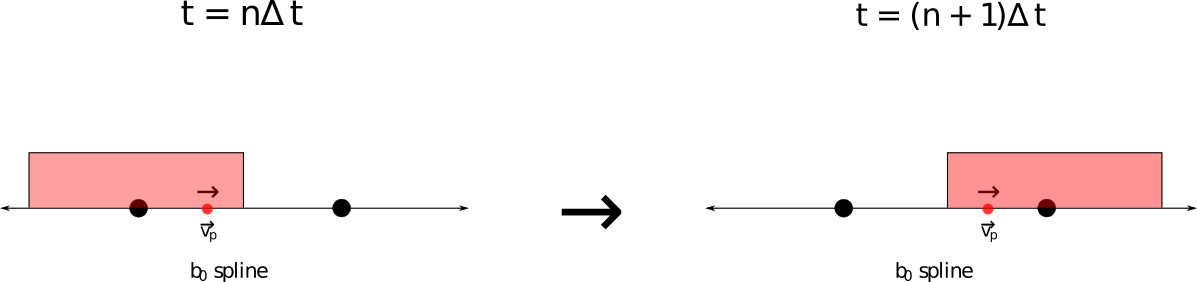
\includegraphics[width=12cm]{extra_credit}
\caption{$b_{0}$ weighted particle viewed by the grid}
\end{figure}

The main advantage of using computational/finite sized particles is the \textbf{nature of interactions between particles at close ranges}. The interpolated electric field acting on the macro particles in the PIC code is Coulombic in nature when the particles are away from each other.  

\begin{figure}[!htb]
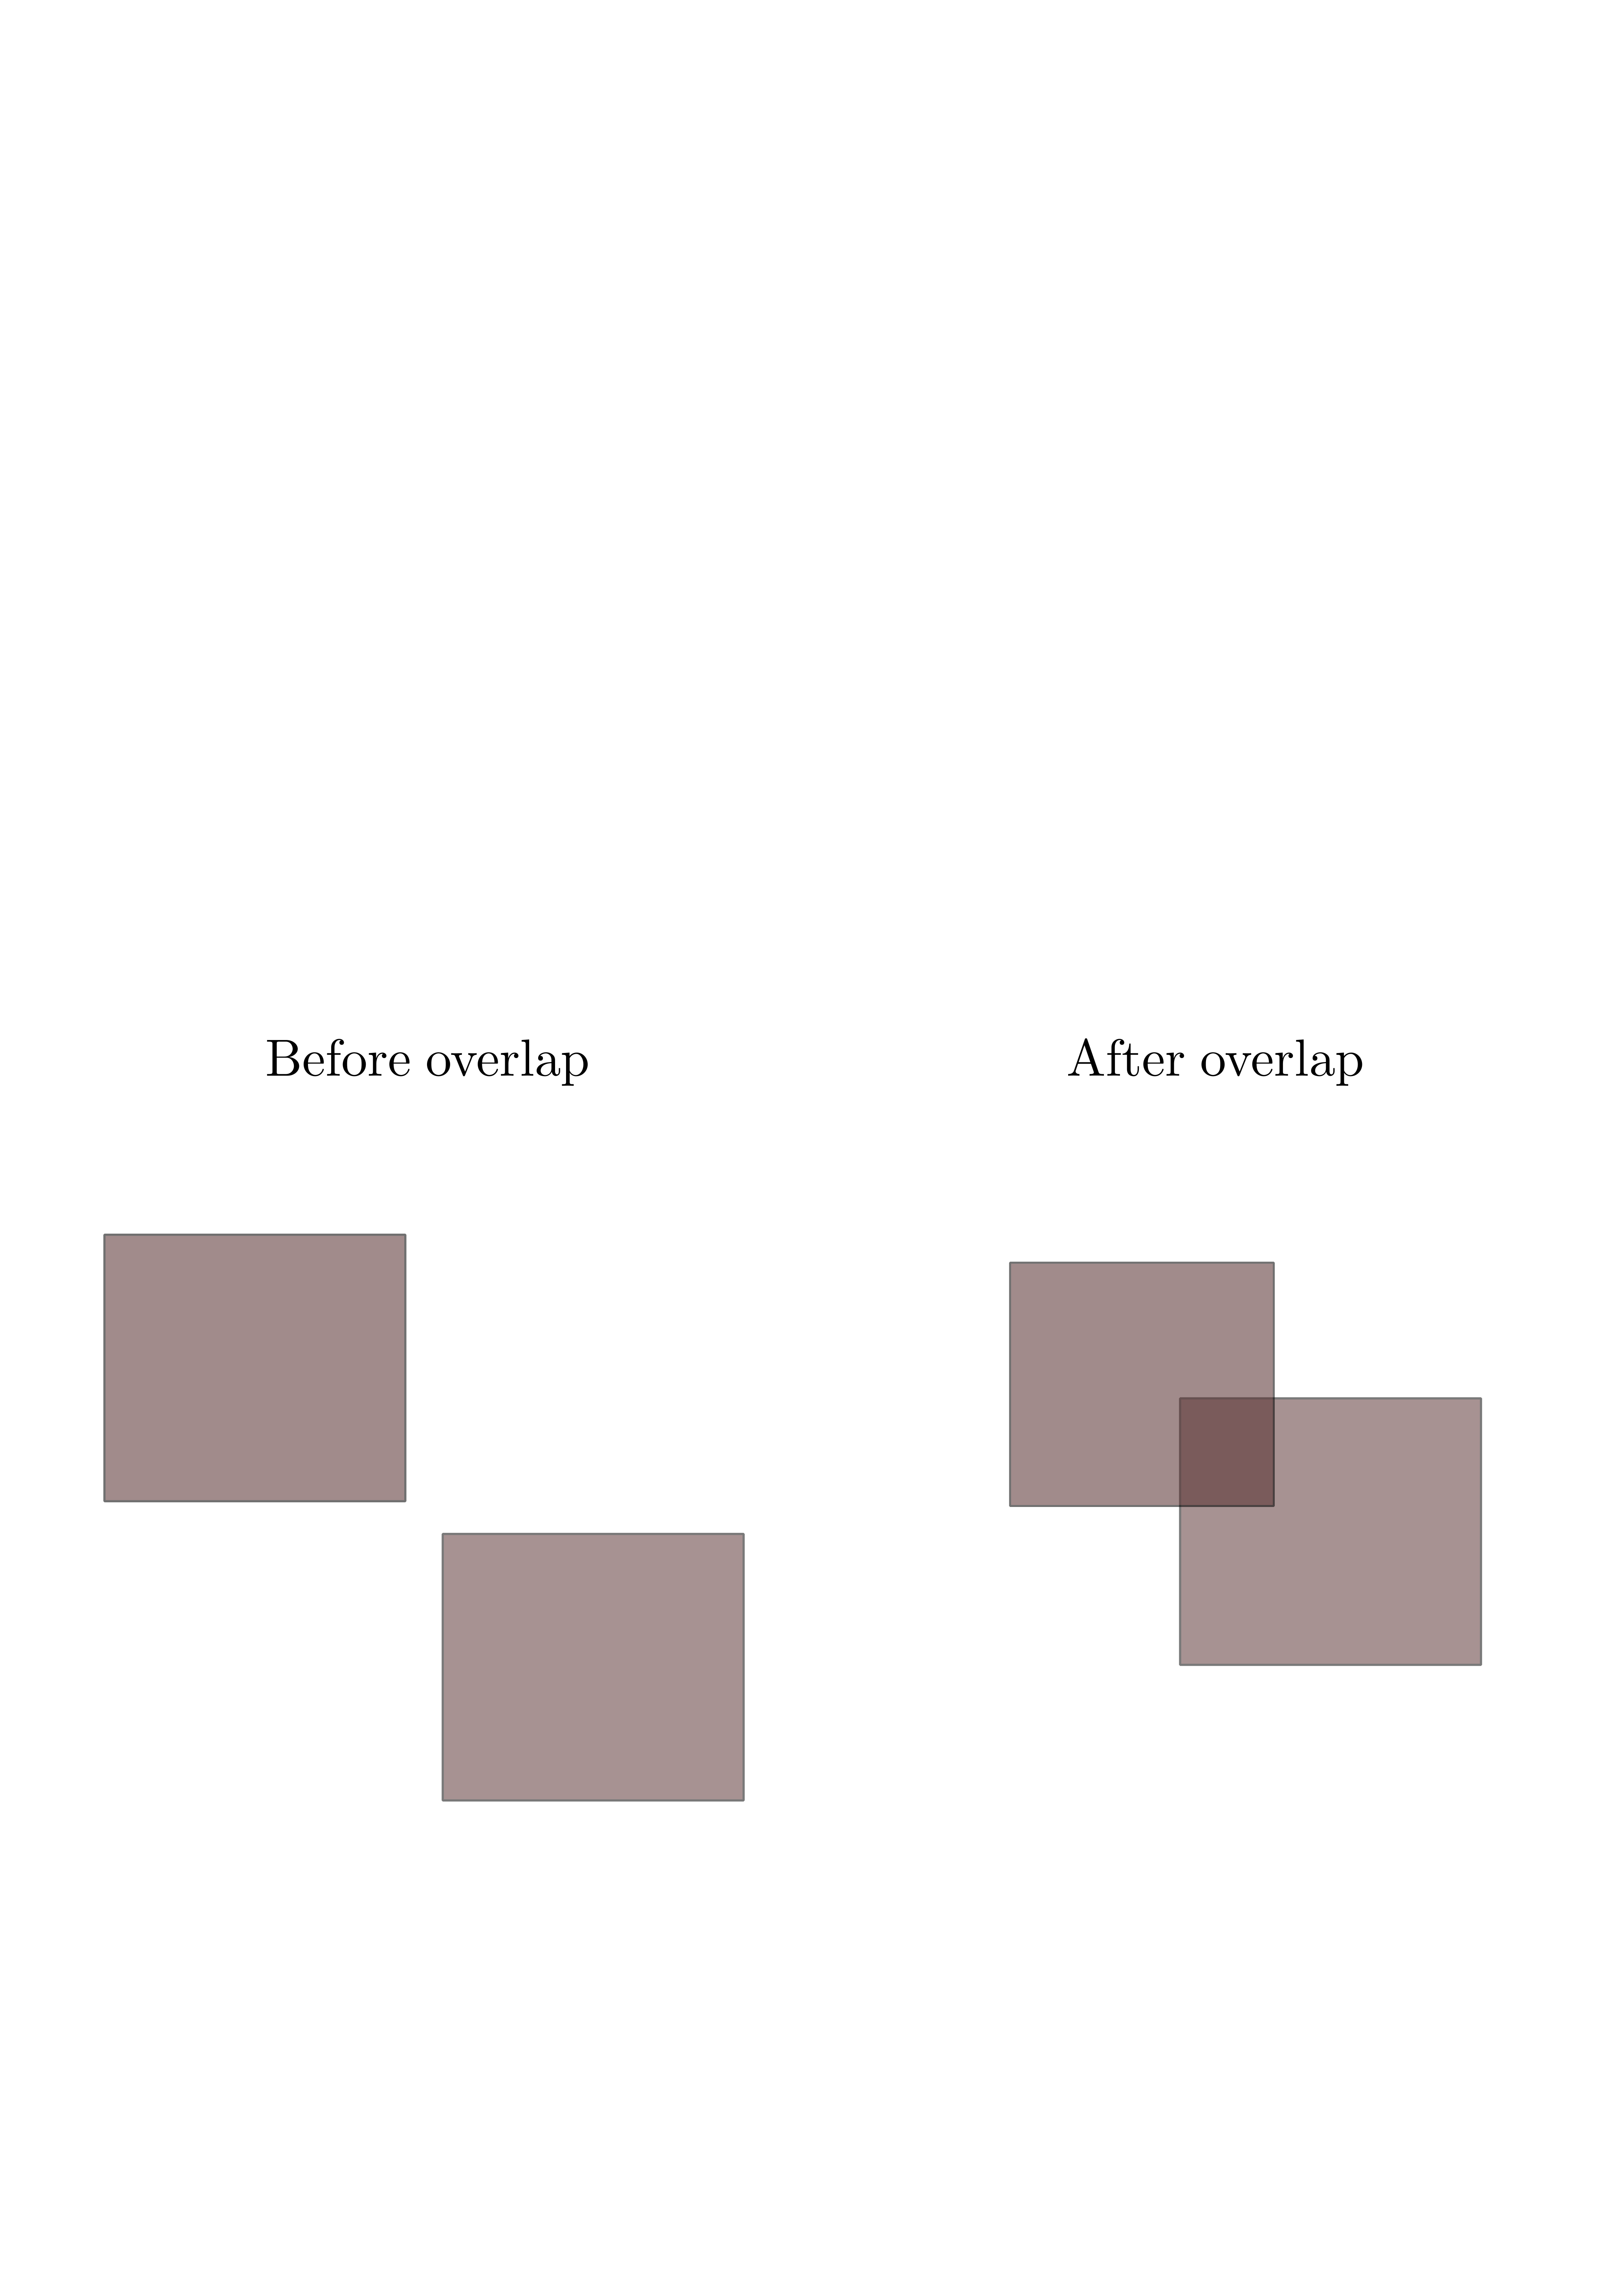
\includegraphics[width=7cm]{finiteParticles}
\caption{Overlap of $b_{0}$ weighted particles viewed by the grid}
\end{figure}

When the two macro particles start approaching each other on the computational grid, the interpolated electric field acting on the particles slowly approaches zero as the macro particles completely overlap each other. This can be verified by taking two particles in the domain with the same position and computing the interpolated electric field acting on the particles in a PIC code. This allows \textbf{macro particles to approach each other with weak interactions between them at close ranges in PIC simulations}. This nature of interaction arises as a \textbf{numerical effect due to non physical grid forces arising due to use of finite support shape factors on a finite grid}. Further details on the same can be found in section 4.8(Page 89) in reference \cite{3}. This make PIC a viable option to study collisionless plasmas as particles can approach each other with relatively weak interactions between them at close ranges. 

The degree of coarse graining or the number of particles represented by the macro particle affects numerical calculations for plasmas with \textbf{collisions or correlations}. \textbf{Study of collisionless plasmas/Vlasov Maxwell system is not affected by the degree of coarse graining}\cite{6}.


\subsection*{Normalizations used in Standard PIC codes}

Normalization used in the PIC code is dependant on user's choice. A suggested normalization scheme is discussed in this section\cite{8,10}.

Quantities of interest in PIC code are namely \textbf{charge ($q$), mass ($m$), Temperature ($T$), distance ($x$), time ($t$), velocity ($v$), Electric field ($E$) and Magnetic field ($B$), number density ($n_{e}$) and current density ($J$).}

Let the normalized quantity of interested quantity $Q$ be denoted by $\bar{Q}$. The table below summarizes the normalization used for the fore-mentioned quantities:

\begin{table}[!htb]
\setlength{\tabcolsep}{0.8em} % for the horizontal padding
{\renewcommand{\arraystretch}{1.8}% for the vertical padding
\begin{tabular}{|c|c|c|}
\hline 
Normalized quantities & Base unit & Evaluation\tabularnewline
\hline 
Charge($\bar{q}$) & e & $\frac{q}{e}$\tabularnewline
Mass($\bar{m}$) & $m_{e}$ &$\frac{m}{m_{e}}$\tabularnewline
distance($\bar{x}$) & $\lambda_{d}$ &$\frac{x}{\lambda_{d}}$\tabularnewline
time($\bar{t}$) & $\omega_{pe}^{-1}$ &$\frac{t}{\omega_{pe}^{-1}}$\tabularnewline
Temperature($\bar{T}$) & $m_{e}c^{2}$ &$\frac{T}{m_{e}c^{2}}$\tabularnewline
Velocity($\bar{v}$) & $c$ &$\frac{v}{c}$\tabularnewline
Electric field($\bar{E}$) & $m_{e}c\omega_{pe}/e$ &$\frac{E}{m_{e}c\omega_{pe}/e}$\tabularnewline
Magnetic field($\bar{B}$) & $m_{e}\omega_{pe}/e$ &$\frac{B}{m_{e}\omega_{pe}/e}$\tabularnewline
Number density($\bar{n_{e}}$) & $\varepsilon_{0}m_{e}\omega_{pe}^{2}/e^{2}$ &$\frac{n_{e}}{\varepsilon_{0}m_{e}\omega_{pe}^{2}/e^{2}}$\tabularnewline
Current density($\bar{J}$) & $en_{e}c$ & $\frac{J}{en_{e}c}$\tabularnewline
\hline 
\end{tabular}
}
\caption{Normalization scheme}
\label{table1}
\end{table}

Where $e$, $m_{e}$, $\omega_{pe}^{-1}$, $T_{eV}$, $v_{th}$, $n_{e}$ and $c$ are the charge of an electron, mass of an electron, plasma period, temperature expressed in energy($K_{B}T$), thermal velocity, average electron density and speed of light respectively. 

The normalization scheme presented in the current section is dependant plasma period (chosen according to the real plasma of interest) is given by the following formula
\begin{align}
\omega_{pe}^{-1} = \sqrt{\frac{m_{e} \varepsilon_{0} }{ \bar{ n_{e}}q_{e}^{2}} }
\end{align}


The temperature is supplied in electron volts which is commonly the norm in plasma physics \cite{9}. This nominal temperature($\bar{T}$) corresponds to $k_{B}T$ of the system of interest. For example, a plasma of 170 Mega Kelvin would correspond to a normalized temperature of 15$eV$. The normalization scheme suggested in this section used the base unit as $m_{e}c^{2}$ instead of electron volts($eV$). 

\textbf{Note:} The normalization scheme presented in this section is used to simulate real plasma's and all the parameters given must correspond to a real plasma of interest. 

All the characteristic quantities of the real plasma are evaluated in S.I or c.g.s units and normalized by dividing the computed values by the respective base unit. These normalized quantities are provided as input to the PIC code. The results generated by the PIC code are brought back to S.I units by multiplying the computed results by their respective base units.

\subsection*{Comparison of Linear theory calculations with PIC}

The distribution function $f(x, v, t)$ used in both PIC and linear theory calculations must be statistically equivalent to compare the results between analytical calculations and particle in cell calculations. 

Let the distribution function in analytical calculations be $f_{a}(x, v, t)$ and $f_{pic}(x, v, t)$ respectively, where $f_{pic}(x, v, t)$ is given as follows:
\begin{align}
f_{pic}(x, v, t) = A\sum_{p=1}^{N_{m}} w_{p}S(x, x_{p})S(v, v_{x,p})
\end{align}

Where $A$ be the normalization factor. The results generated by the PIC code or analytical codes is normalized to draw a comparison between the results. The normalization factor for comparing the analytical and PIC results is given as follows:
\begin{align}
f_{pic} &= f_{a}  \\
\implies A &= \frac{\int \int f_{a}\;dv\;dx}{\int \int f_{pic}\;dv\;dx}  \\
A &= \frac{\int \int f_{a}\;dv\;dx}{\int \int\sum_{p=1}^{N_{m}} w_{p}S(x, x_{p})S(v, v_{x,p})\;dv\;dx} \\
A &= \frac{\int \int f_{a}\;dv\;dx}{N_{m} * w_{p}}
\end{align}





\medskip
 
\begin{thebibliography}{7}
\bibitem{1} 
DOI: 10.13140/RG.2.1.3319.2801. Conference: XII Carolus Magnus Summer School on Plasma and Fusion Energy Physics
\bibitem{2}
\url{http://theory.ipp.ac.cn/~yj/research_notes/particle_simulation.pdf}
\bibitem{3}
Charles K. Birdsall, A.Bruce Langdon-Plasma physics via computer simulation-McGraw-Hill (1991)
\bibitem{4}
\url{http://www.tp1.ruhr-uni-bochum.de/~grauer/lectures/CompII/PIClecture}
\bibitem{5}
\url{http://theory.ipp.ac.cn/~yj/research_notes/particle_simulation.pdf}
\bibitem{6}
\url{https://arxiv.org/abs/1311.4709}
\bibitem{7}
\url{https://publishup.uni-potsdam.de/opus4-ubp/files/7453/wieland_diss.pdf}
\bibitem{8}
\url{http://ssl.mit.edu/files/website/theses/PhD-2001-SzaboJames.pdf}
\bibitem{9}
\url{https://en.wikipedia.org/wiki/Electronvolt#Temperature}
\bibitem{10}
\url{https://arxiv.org/pdf/1702.05128.pdf}
\end{thebibliography}
\end{document}